\chapter{Ambito dell'elaborato e del progetto}
\label{cha:ambito}
Questo capitolo ha lo scopo di illustrare ad alto livello il lavoro svolto durante il tirocinio riguardante la progettazione e l'implementazione del software gestionale aziendale. In particolare si riportano, in modo più astratto, alcuni temi legati ai Sistemi Informativi \cite{SI} e alla gestione dei processi delle organizzazioni. I capitoli successivi, invece, entrano maggiormente nei dettagli di analisi e sviluppo tecnico.\newline
Di seguito si introducono argomenti relativi ai profili informativi, alla potenzialità e attrattività informatica e alla costruzione di un sistema informativo, presentando prima una breve spiegazione del tema e specificando poi il posizionamento del documento rispetto al concetto espresso.   

\subsection{L'esigenza informativa}
\label{sec:anthony}
Il ruolo principale di ogni sistema informativo è quello di fornire aiuto e supporto alla gestione aziendale aumentando il livello di astrazione con l'aumentare del livello decisionale.
Le operazioni svolte possono essere classificate in base alle attività compiute e ai requisiti richiesti dai vari attori che lavorano dell'organizzazione. Per rappresentare questa divisione si fa spesso riferimento alla Piramide di Anthony \cite{anthony}\cite{anthony2} (figura \ref{fig:anthony}), schema composto da tre livelli, ognuno dei quali svolge incarichi differenti e possiede un profilo informativo diverso assegnato. Il livello base riguarda infatti il personale esecutivo con attività operative, la parte intermedia dello schema coinvolge la direzione funzionale con attività tattiche, mentre la punta della piramide riguarda i processi dell'alta direzione con i ruoli più strategici.
\begin{figure}[!hbt]
\centering
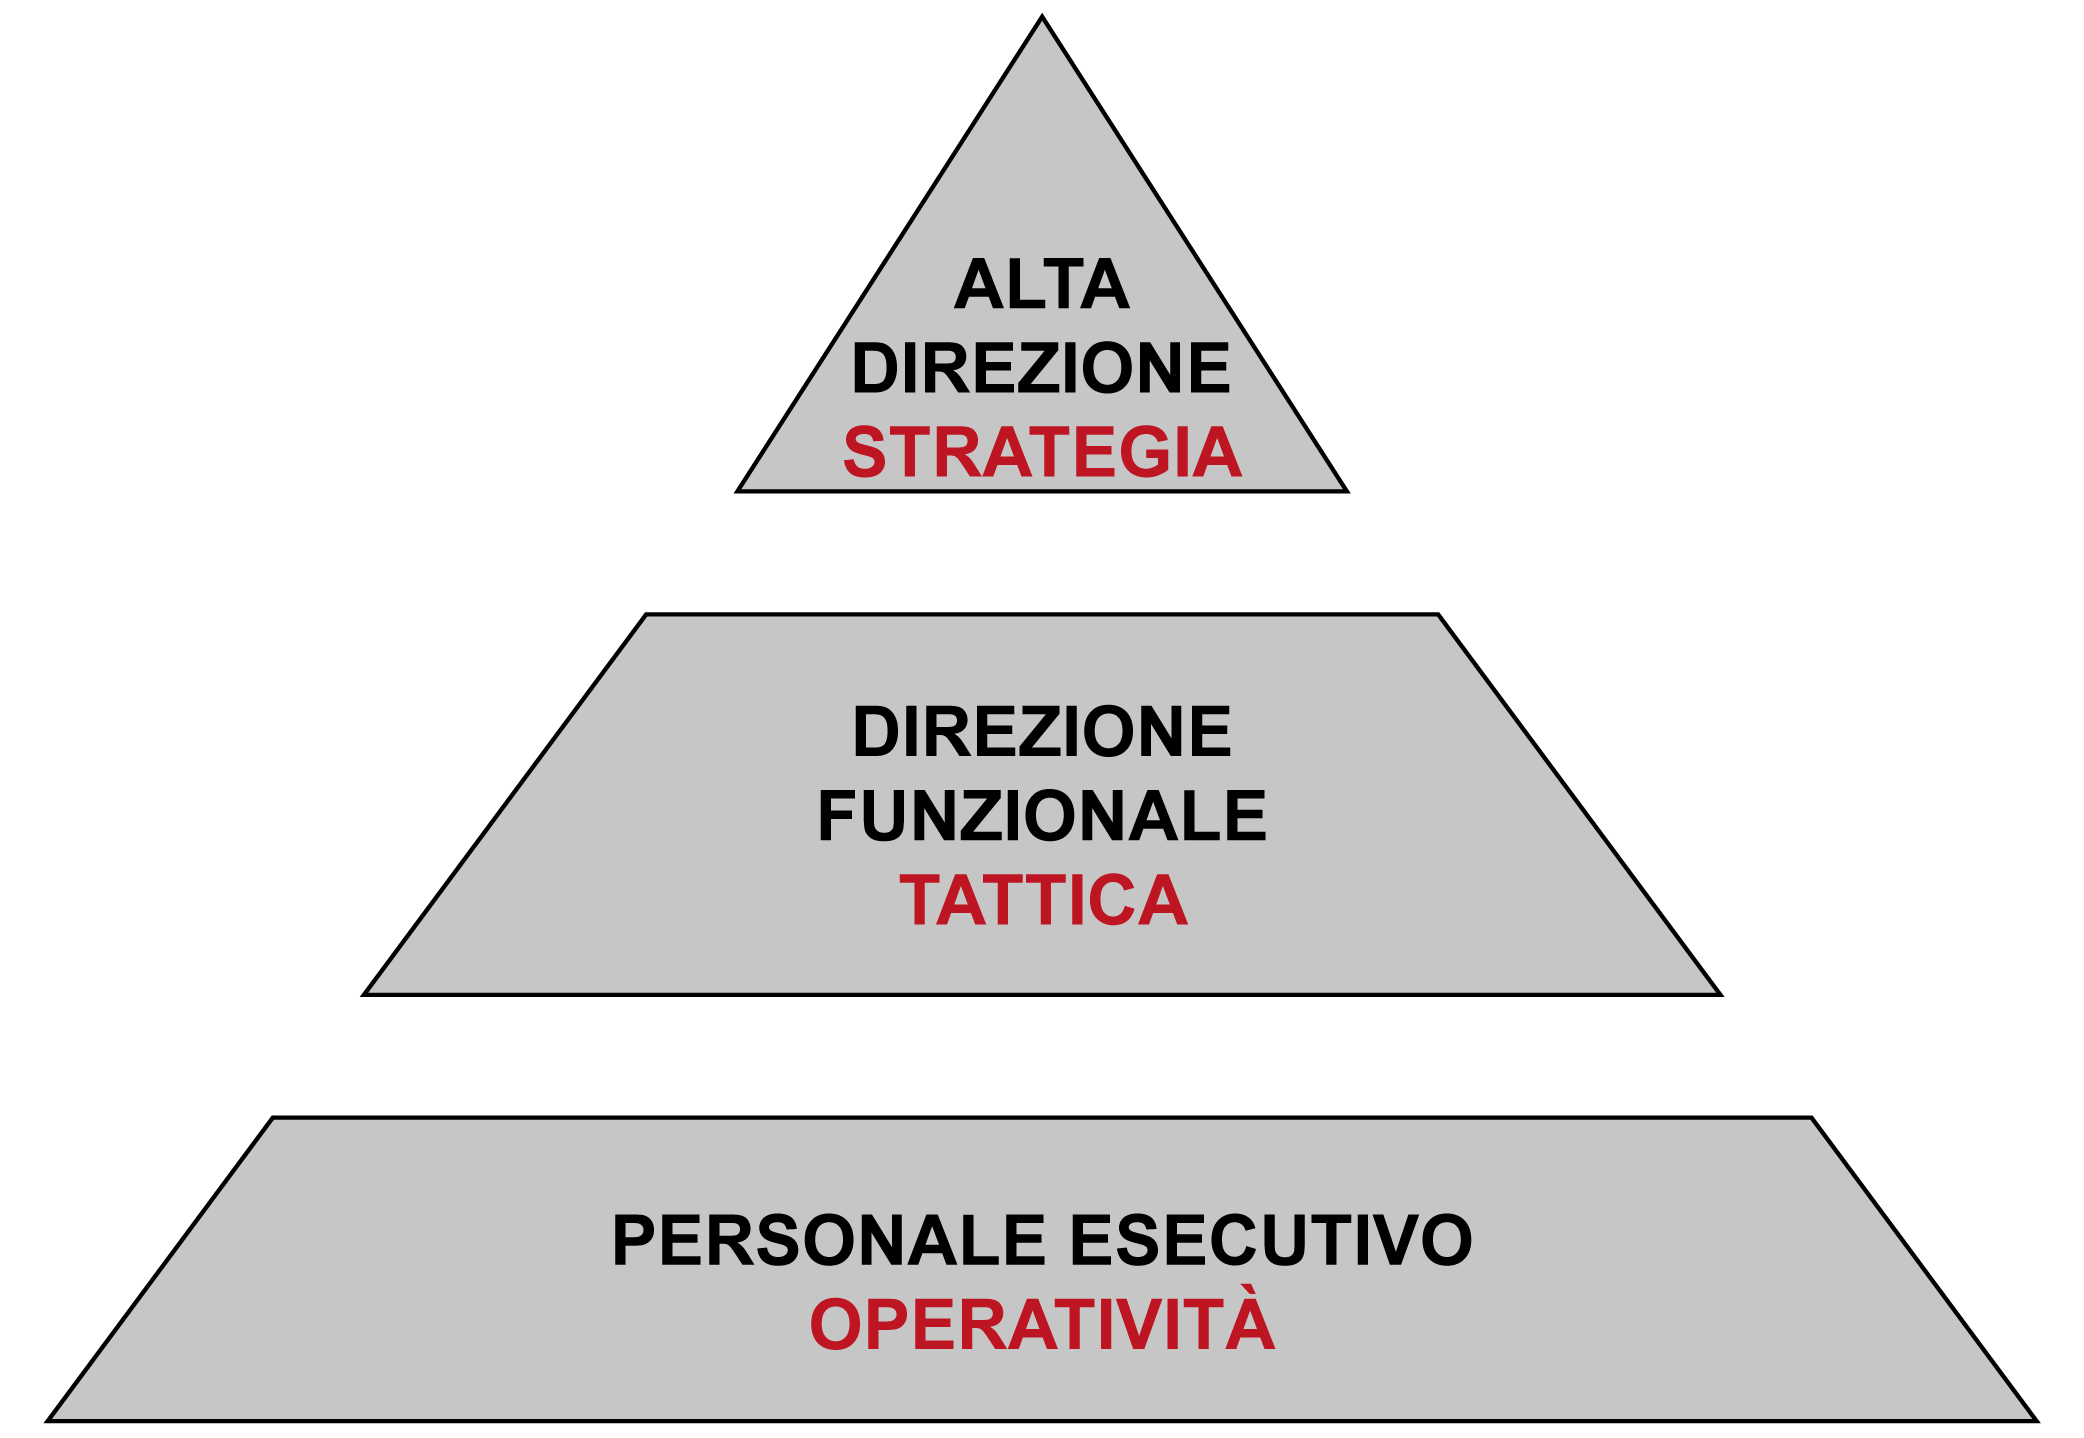
\includegraphics[scale=0.45]{img/anthony_scheme.png}
\caption{Piramide di Anthony}
\label{fig:anthony}
\end{figure}
\newline
\noindent
I processi trattati e analizzati nel progetto seguito si collocano a livello operativo che lavora con grandi volumi di dati precisi, analitici e interni all'azienda, con frequenza continua. Queste attività richiedono informazioni dettagliate ed esatte, fornite con tempestività; raramente si opera con dati sintetici. \\
\newline
Per quanto riguarda la scomposizione del sistema informativo, la collocazione dei processi implementati ricade sul sistema operazionale (e non su quello informazionale). Le funzioni principali sono perciò quelle di aiutare l'azienda nell'automatizzare tutte le operazioni procedurali dell'area coinvolta, definire e integrare nuovi processi e rendere guidate e strutturate le attività esecutive. L'obiettivo è pertanto quello di permettere l'accesso alle informazioni attuali in modo interattivo, con la possibilità di leggere, modificare ed inserire nuovi dati. Questi tipi di sistemi usano un database operazionale \cite{operational_database} e una serie di metodi operativi per rendere possibile un'analisi OLTP (On Line Transaction Processing) \cite{oltp}. L'elaborazione dei dati prevede l'esecuzione di molte transizioni contemporanee di vari utenti che accedono alla base di dati effettuando ricerche e/o modifiche, e garantisce in qualsiasi momento l'accesso alle informazioni in modo coerente e corretto.

\subsection{L'attrattività informatica}
\label{sec:attrattivita}
I sistemi operazionali hanno come obiettivo principale quello di permettere la pianificazione e il controllo dei processi coinvolti, con conseguente acquisizione e organizzazione della conoscenza e delle situazioni dell'impresa. Per questo motivo è spesso utile definire quella che viene considerata la ``potenzialità informatica'' di un'azienda. Questo concetto viene influenzato da vari fattori come la propensione all'uso e all'implementazione di strutture tecnologiche e informatiche a sostegno delle attività, l'intensità informativa (definito dalla struttura dell'organizzazione e dalla quantità di informazioni necessarie) e l'attrattività informatica.
Quest'ultimo parametro è legato al grado di efficacia, facilità e competenza nel rendere informatizzato un processo aziendale.\\
\begin{figure}[!hbt]
\centering
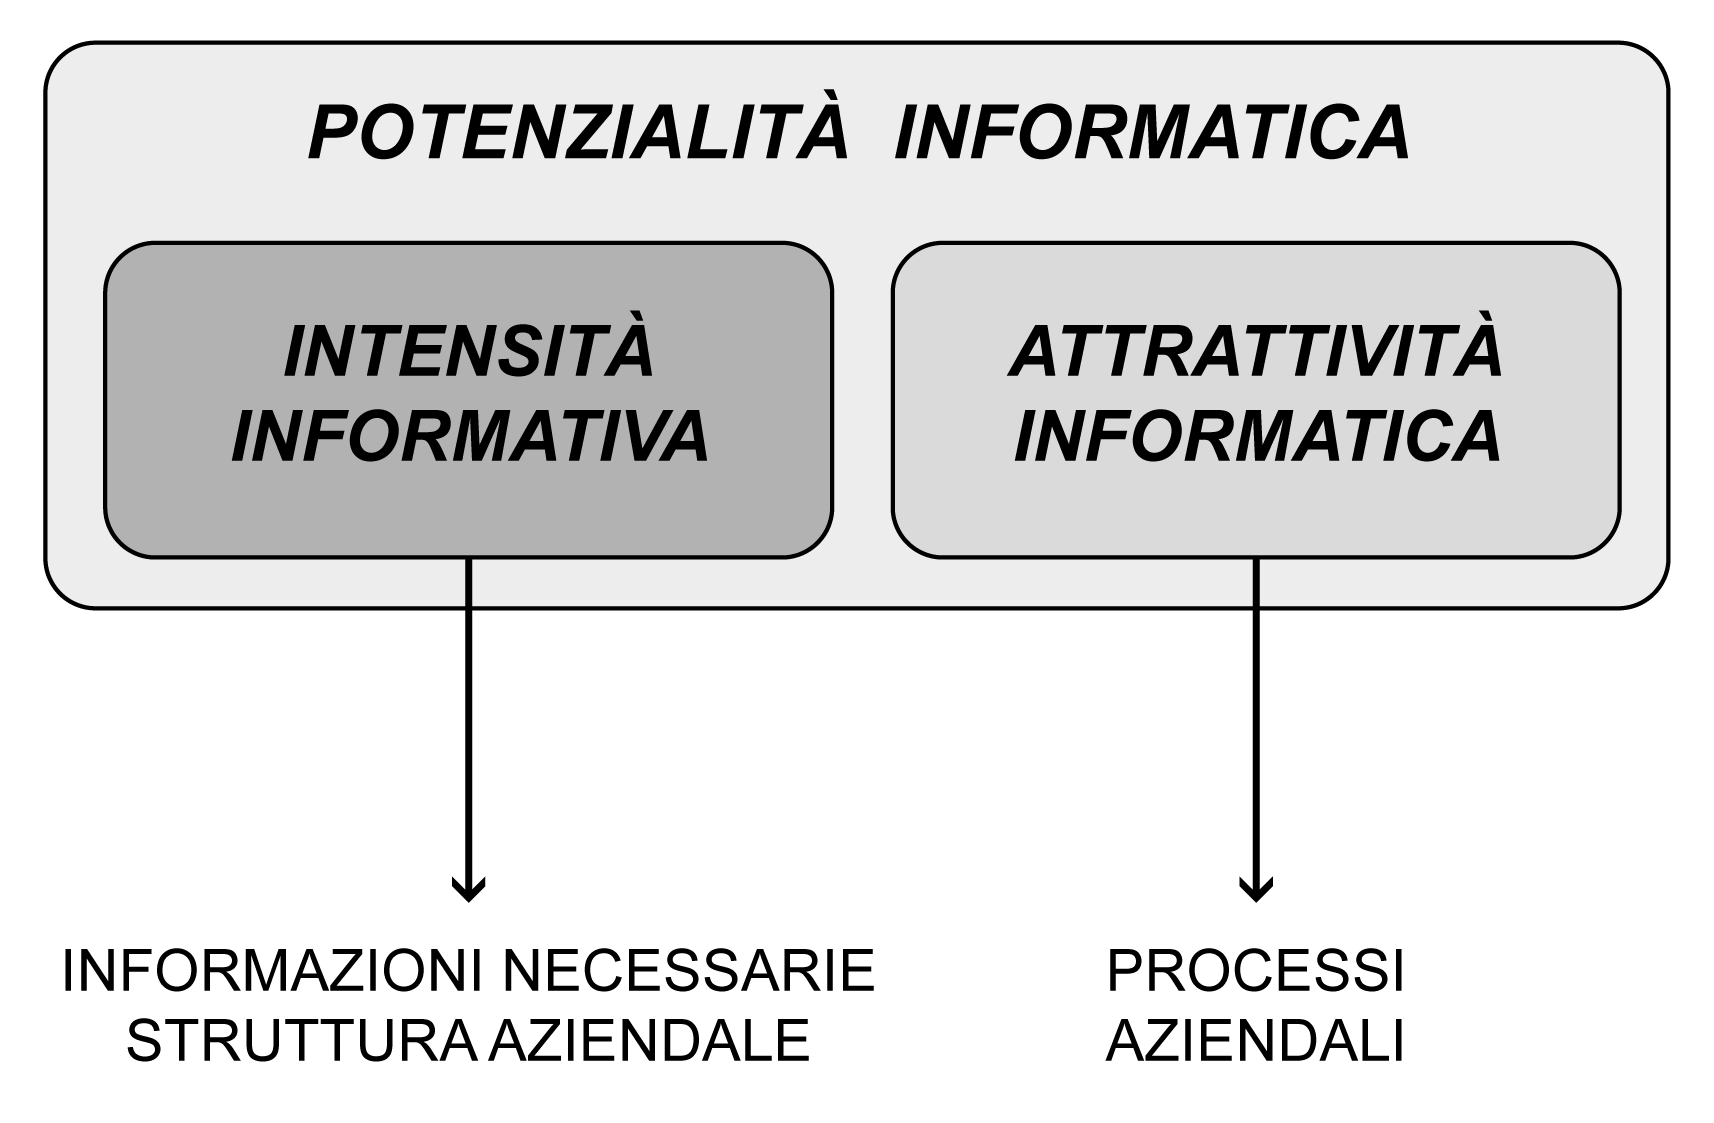
\includegraphics[scale=0.55]{img/potenzialita.png}
\caption{Potenzialità Informatica}
\label{fig:potenzialita}
\end{figure}
\noindent
\newline
La necessità di sviluppare il gestionale richiesto è stata ponderata in base proprio all'elevata attrattività informatica di tutti i processi coinvolti in questo progetto. Questa esigenza è stata determinata dall'elevato grado procedurale, ovvero di strutturazione dei flussi coinvolti e dall'alta ripetitività, intesa come la frequenza di ripetizione nel tempo di una sequenza di operazioni senza particolari modifiche. Inoltre, dati gli elevati volumi di informazioni da elaborare e il basso o medio grado di difficoltà di molte azioni elementari del processo, è evidente l'elevata attrattiva informatica dell'intero applicativo richiesto; a questo si aggiungono anche la buona propensione e le abitudini delle figure interne all'azienda nell'usare già sistemi informatici per altri processi.      
\begin{figure}[!hbt]
\centering
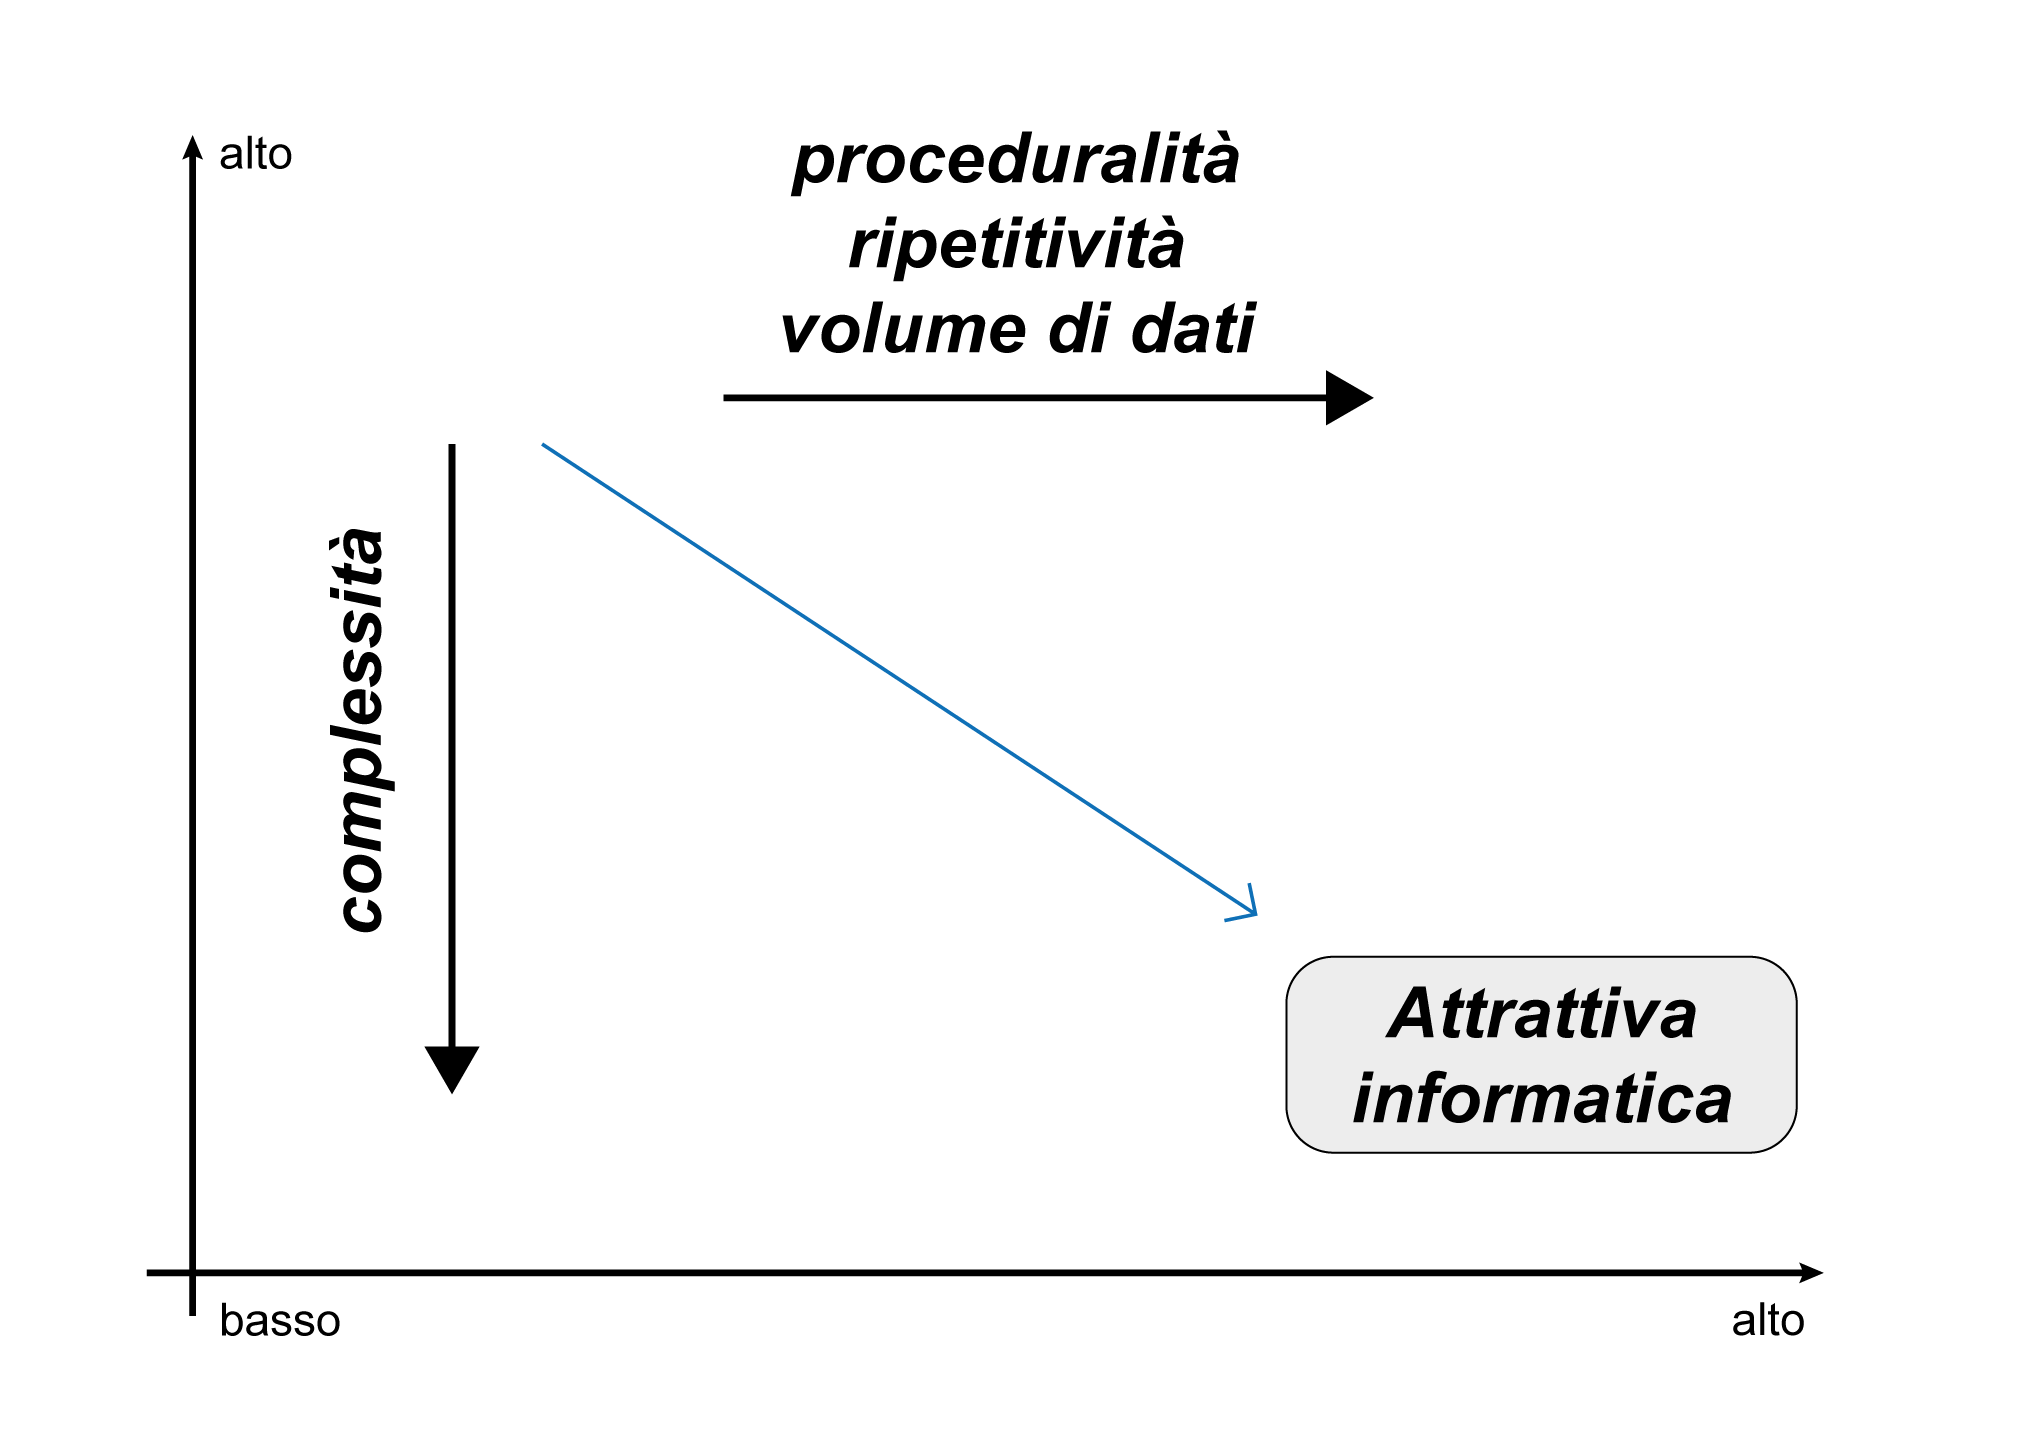
\includegraphics[scale=0.55]{img/attrattiva.png}
\caption{Attrattiva Informatica}
\label{fig:attrattiva}
\end{figure}
\noindent
\newline


\subsection{Costruzione del Sistema Informativo}
\label{sec:make}
Durante la fase di digitalizzazione dei processi e, quindi, di costruzione del Sistema Informativo, ogni azienda è tenuta a prendere una decisione in termini di possibili percorsi da seguire, scegliendo tra:
\begin{itemize}
    \item \textit{Make}
    \item \textit{Buy}
    \item \textit{Outsource}
\end{itemize}
La prima opzione consiste, in sintesi, nel costruire tutti gli applicativi e servizi del Sistema Informativo in modo interno e autonomo, presupponendo la presenza di un gruppo di lavoro in grado non solo di progettare il sistema nel presente, ma anche di mantenerlo nel tempo. La scelta di acquisto invece prevede di comprare il software da fornitori esterni; è la scelta più comune nelle piccole e medie imprese in quanto richiede solo di avere delle figure per gestire gli utenti interni e comunicare con i tecnici distributori. Nonostante la maggior flessibilità rispetto all'opzione \textit{Make} e il vantaggio in termini di confronto con il mercato, l'organizzazione è totalmente dipendente da una struttura esterna. L'ultima possibilità è quella di affidare la gestione e l'organizzazione del Sistema Informativo a un ente  esterno; questa scelta sta diventando sempre più popolare in quanto, a fronte di un canone periodico, costi più bassi, garanzie di sicurezza e di connettività si uniscono alla flessibilità interna e ai vantaggi del \textit{Buy}. Si deve però accettare la perdita di controllo su un elemento molto importante del modello organizzativo aziendale.
\begin{figure}[!hbt]
\centering
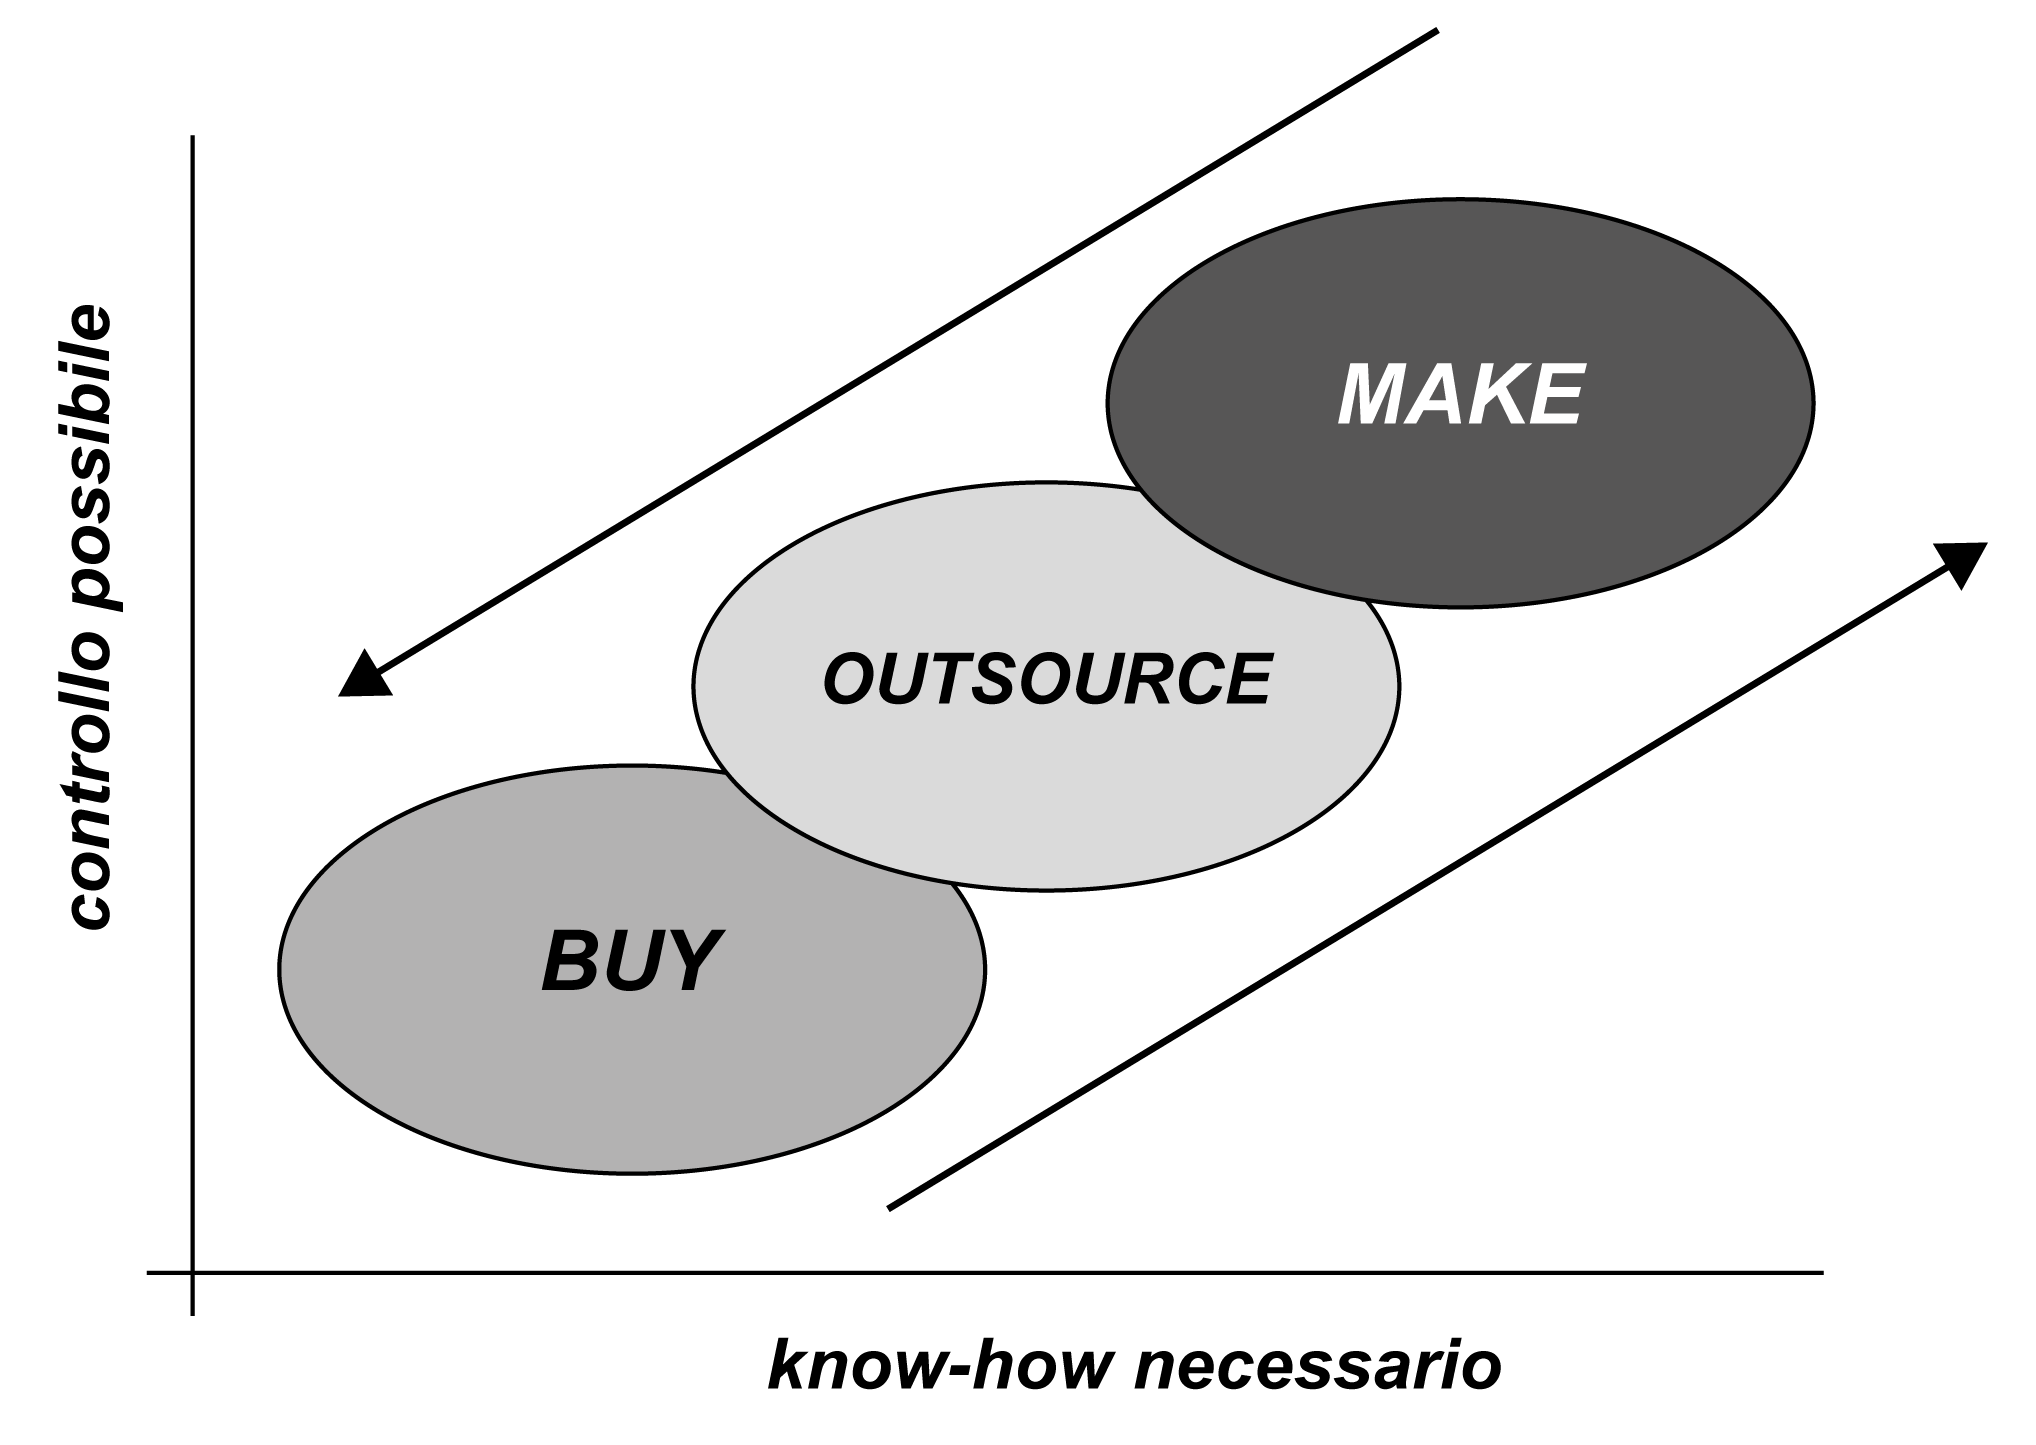
\includegraphics[scale=0.55]{img/makevsbuy.png}
\caption{Costruzione del SI: le possibilità}
\label{fig:makevsbuy}
\end{figure}
\newline
\noindent
Una volta individuati, se pur ad alto livello, i processi interessati da automatizzare, nella prima fase del tirocinio si sono analizzati con precisione tutti i vantaggi e le conseguenze di ognuna delle opzioni disponibili elencate per l'implementazione del software richiesto. Dopo una primo periodo di ricerca sul mercato di possibili soluzioni acquistabili che rispettassero i requisiti stabiliti, si è arrivati alla conclusione di scegliere l'approccio \textit{Make} per ottenere una mappatura puntuale e su misura del modello organizzativo in questione. Si è infatti considerata la complessità relativamente contenuta, almeno per una prima versione base del gestionale, e la necessità di avere un'automatizzazione dei flussi di lavoro per lo più personalizzati e ``ad hoc''. La soluzione di produrre interamente un applicativo o un servizio rappresenta, per la maggior parte delle PMI, una scelta non comune, dati gli investimenti necessari generalmente elevati e la mancanza di inserimento e confronto con il mercato. Al contrario, in questo specifico caso, è risultato vantaggioso creare il gestionale internamente grazie ai costi pressoché nulli e al know-how aziendale già presente.              
\clearpage
\newpage